% Options for packages loaded elsewhere
\PassOptionsToPackage{unicode}{hyperref}
\PassOptionsToPackage{hyphens}{url}
\PassOptionsToPackage{dvipsnames,svgnames,x11names}{xcolor}
%
\documentclass[
  number]{elsarticle}

\usepackage{amsmath,amssymb}
\usepackage{iftex}
\ifPDFTeX
  \usepackage[T1]{fontenc}
  \usepackage[utf8]{inputenc}
  \usepackage{textcomp} % provide euro and other symbols
\else % if luatex or xetex
  \usepackage{unicode-math}
  \defaultfontfeatures{Scale=MatchLowercase}
  \defaultfontfeatures[\rmfamily]{Ligatures=TeX,Scale=1}
\fi
\usepackage{lmodern}
\ifPDFTeX\else  
    % xetex/luatex font selection
\fi
% Use upquote if available, for straight quotes in verbatim environments
\IfFileExists{upquote.sty}{\usepackage{upquote}}{}
\IfFileExists{microtype.sty}{% use microtype if available
  \usepackage[]{microtype}
  \UseMicrotypeSet[protrusion]{basicmath} % disable protrusion for tt fonts
}{}
\makeatletter
\@ifundefined{KOMAClassName}{% if non-KOMA class
  \IfFileExists{parskip.sty}{%
    \usepackage{parskip}
  }{% else
    \setlength{\parindent}{0pt}
    \setlength{\parskip}{6pt plus 2pt minus 1pt}}
}{% if KOMA class
  \KOMAoptions{parskip=half}}
\makeatother
\usepackage{xcolor}
\setlength{\emergencystretch}{3em} % prevent overfull lines
\setcounter{secnumdepth}{5}
% Make \paragraph and \subparagraph free-standing
\makeatletter
\ifx\paragraph\undefined\else
  \let\oldparagraph\paragraph
  \renewcommand{\paragraph}{
    \@ifstar
      \xxxParagraphStar
      \xxxParagraphNoStar
  }
  \newcommand{\xxxParagraphStar}[1]{\oldparagraph*{#1}\mbox{}}
  \newcommand{\xxxParagraphNoStar}[1]{\oldparagraph{#1}\mbox{}}
\fi
\ifx\subparagraph\undefined\else
  \let\oldsubparagraph\subparagraph
  \renewcommand{\subparagraph}{
    \@ifstar
      \xxxSubParagraphStar
      \xxxSubParagraphNoStar
  }
  \newcommand{\xxxSubParagraphStar}[1]{\oldsubparagraph*{#1}\mbox{}}
  \newcommand{\xxxSubParagraphNoStar}[1]{\oldsubparagraph{#1}\mbox{}}
\fi
\makeatother


\providecommand{\tightlist}{%
  \setlength{\itemsep}{0pt}\setlength{\parskip}{0pt}}\usepackage{longtable,booktabs,array}
\usepackage{calc} % for calculating minipage widths
% Correct order of tables after \paragraph or \subparagraph
\usepackage{etoolbox}
\makeatletter
\patchcmd\longtable{\par}{\if@noskipsec\mbox{}\fi\par}{}{}
\makeatother
% Allow footnotes in longtable head/foot
\IfFileExists{footnotehyper.sty}{\usepackage{footnotehyper}}{\usepackage{footnote}}
\makesavenoteenv{longtable}
\usepackage{graphicx}
\makeatletter
\def\maxwidth{\ifdim\Gin@nat@width>\linewidth\linewidth\else\Gin@nat@width\fi}
\def\maxheight{\ifdim\Gin@nat@height>\textheight\textheight\else\Gin@nat@height\fi}
\makeatother
% Scale images if necessary, so that they will not overflow the page
% margins by default, and it is still possible to overwrite the defaults
% using explicit options in \includegraphics[width, height, ...]{}
\setkeys{Gin}{width=\maxwidth,height=\maxheight,keepaspectratio}
% Set default figure placement to htbp
\makeatletter
\def\fps@figure{htbp}
\makeatother

\makeatletter
\@ifpackageloaded{caption}{}{\usepackage{caption}}
\AtBeginDocument{%
\ifdefined\contentsname
  \renewcommand*\contentsname{Table of contents}
\else
  \newcommand\contentsname{Table of contents}
\fi
\ifdefined\listfigurename
  \renewcommand*\listfigurename{List of Figures}
\else
  \newcommand\listfigurename{List of Figures}
\fi
\ifdefined\listtablename
  \renewcommand*\listtablename{List of Tables}
\else
  \newcommand\listtablename{List of Tables}
\fi
\ifdefined\figurename
  \renewcommand*\figurename{Figure}
\else
  \newcommand\figurename{Figure}
\fi
\ifdefined\tablename
  \renewcommand*\tablename{Table}
\else
  \newcommand\tablename{Table}
\fi
}
\@ifpackageloaded{float}{}{\usepackage{float}}
\floatstyle{ruled}
\@ifundefined{c@chapter}{\newfloat{codelisting}{h}{lop}}{\newfloat{codelisting}{h}{lop}[chapter]}
\floatname{codelisting}{Listing}
\newcommand*\listoflistings{\listof{codelisting}{List of Listings}}
\makeatother
\makeatletter
\makeatother
\makeatletter
\@ifpackageloaded{caption}{}{\usepackage{caption}}
\@ifpackageloaded{subcaption}{}{\usepackage{subcaption}}
\makeatother
\ifLuaTeX
  \usepackage{selnolig}  % disable illegal ligatures
\fi
\usepackage[]{natbib}
\bibliographystyle{elsarticle-num}
\usepackage{bookmark}

\IfFileExists{xurl.sty}{\usepackage{xurl}}{} % add URL line breaks if available
\urlstyle{same} % disable monospaced font for URLs
\hypersetup{
  pdftitle={Mapping landscape suitability for forest thinning to reduce evapotranspiration and enhance groundwater recharge in Arizona},
  pdfauthor={Ryan E Lima; Neha Gupta; Travis Zalesky; Temuulen Tsagaan Sankey; Abraham E Springer; Katherine Jacobs},
  pdfkeywords={suitability mapping, Forest thinning, Water
yield, groundwater recharge, GIS-MCDM, AHP},
  colorlinks=true,
  linkcolor={blue},
  filecolor={Maroon},
  citecolor={Blue},
  urlcolor={Blue},
  pdfcreator={LaTeX via pandoc}}

\setlength{\parindent}{6pt}
\begin{document}

\begin{frontmatter}
\title{Mapping landscape suitability for forest thinning to reduce
evapotranspiration and enhance groundwater recharge in Arizona}
\author[1]{Ryan E Lima%
\corref{cor1}%
}
 \ead{ryan.lima@nau.edu} 
\author[2]{Neha Gupta%
%
}

\author[2]{Travis Zalesky%
%
}

\author[1]{Temuulen Tsagaan Sankey%
%
}

\author[1]{Abraham E Springer%
%
}

\author[2]{Katherine Jacobs%
%
}


\affiliation[1]{organization={Northern Arizona
University},,postcodesep={}}
\affiliation[2]{organization={University of Arizona},,postcodesep={}}

\cortext[cor1]{Corresponding author}






        
\begin{abstract}
Literature on the relationship between forest thinning and water yield
was used to develop suitability criteria to map where forest treatment
is most likely to enhance groundwater recharge across the Mogollon Rim
Ranger District in the Coconino National Forest. Rechage in the region
is ephemeral and focused in periods of snowmelt and locations of
enhanced permeability when soil moisture exceeds threshold levels. Our
approach combines thematic maps of criteria such as average
precipitation, snow dominance, slope, aspect,landscape morphology,
forest density, lithology and hydrologic soil type into a
GIS-Multi-Criteria Decision Making model. Pairwise comparisons were made
between criteria, and Analytic Hierachy Process was used as a weighting
method.
\end{abstract}





\begin{keyword}
    suitability mapping \sep Forest thinning \sep Water
yield \sep groundwater recharge \sep GIS-MCDM \sep 
    AHP
\end{keyword}
\end{frontmatter}
    
\section{Introduction}\label{introduction}

Since 2000, the Colorado River Basin has been in the midst of a historic
drought \citep{meko_treering_2022, williams_rapid_2022}. Average
temperatures increased by 0.9ºC from 2000 - 2014, and streamflow in the
Colorado River has declined by 19\% below the 1906-1999 average
\citep{hogan_recent_2024, udall_twentyfirst_2017}. Extreme hydroclimate
events such as droughts, heatwaves, and floods have more than doubled in
frequency since 2010 \citep{bennett_concurrent_2021}. Simultaneously,
like much of the inter-mountain west, Arizona has experienced rapid
population growth, increasing the demands on already strained water
supplies. Reductions in streamflow have increased reliance on
groundwater pumping, while groundwater levels have declined for decades
in much of the state \citep{tadych_historical_2024}.

Concurrently, western forests are at increasing risk from catastrophic
wildfires--an emerging driver of runoff change that will increase the
impact on the water supply \citep{williams_rapid_2022}. Forest structure
in the Ponderosa Pine forests of Northern Arizona and New Mexico has
changed significantly post-Euro-American settlement due to grazing,
logging, wildfire exclusion, and other factors
\citep{covington_southwestern_1994, friederici2013}. As a result, many
forests are overstocked relative to pre-settlement conditions,
increasing the risk of catastrophic wildfire
\citep{allen_ecological_2002}. Rising temperatures and related droughts
have contributed to extensive tree mortality from wildfire, disease, and
insect infestation \citep{berner_tree_2017}. Warming temperatures have
tripled the frequency and quadrupled the size of wildfires in recent
decades \citep{williams_rapid_2022}. Increasing heat has pushed many
low-elevation conifer forests past climate thresholds, creating
conditions less suitable for tree regeneration
\citep{davis_wildfires_2019}.

Landscape-scale forest restoration efforts have been planned or
implemented across much of Arizona. For example, the Four Forest
Restoration Initiative (4FRI) includes plans for restoration across over
1 million hectares of Arizona's forests
\citep{schultz_collaborative_2012}. The primary goal of restoration
efforts is to reduce wildfire risk
\citep{allen_ecological_2002, friederici2013}. However, numerous studies
have linked forest treatments to increased water yields in semi-arid
forests and have emphasized the role of forest restoration in improving
hydrologic services and increasing water availability
\citep{bosch_review_1982, baker_effects_1986, gottfried_moderate_1991, smerdon_overview_2009, zou_streamflow_2010, wyatt_estimating_2013, moreno_modeling_2015, simonit_impact_2015, wyatt_semiarid_2015, odonnell_forest_2018, schenk_impacts_2020, hibbert1979}.

The connection between forests and water supplies is well documented.
Around 65\% of surface water in the western states originates from
forested lands, which cover just 29\% of the land area
\citep{brown_source_2005}. The average annual precipitation in the Lower
Colorado River Basin is about 330 \(mm\), and only about 10 \(mm\) of
that precipitation becomes streamflow, while much of the rest is lost to
evapotranspiration \citep{zou_streamflow_2010}. Regional studies have
found that up to 90\% of annual precipitation in semi-arid forests is
lost evapotranspiration
\citep{dore_recovery_2012, ha_evapotranspiration_2015, yaseef_ecohydrology_2010, hibbert1979}.
Sublimation has been shown to remove 10 - 90\% of snowfall in the
Colorado River Basin, while the remaining snowmelt provides over 80\% of
streamflow to the Colorado River \citep{lundquist_sublimation_2024}.
Over half of streamflow from the Upper Colorado River basin comes from
groundwater sources primarily recharged by snowmelt \citep{miller2016}.
Therefore, small reductions in evaporative losses could have out-sized
impacts on available water supplies, particularly enhancing groundwater
recharge in terrains underlain by karst lithology
\citep{hibbert1979, wyatt2013}.

While the connection between forest treatment and water yield is well
documented, the response of forests to treatments is complex and
non-linear and differs across forest types, with treatment level, and
along aspect and elevational gradients
\citep{del_campo_global_2022, biederman_streamflow_2022, zou_streamflow_2010, hibbert1979, moore_physical_2005}.
Regardless of the potential for increased water yield the enhancement of
groundwater recharge rarely, if ever, ranks among the primary
motivations for forest treatment
\citep{stanturf2014, filoso2017, allen_ecological_2002, friederici2013}.
This study examines forest restoration through the lens of groundwater
recharge enhancement and identifying potential recharge zones. All else
held equal, we map suitability for forest thinning with the goal of
enhancing recharge. Suitability maps like these may complement (or
supplement) existing frameworks for prioritizing landscape-scale forest
management.

Suitability mapping, and particularly GIS-based Multi-criteria decision
making (GIS-MCDM), is widely used to map potential recharge zones and
areas suitable for Managed Aquifer Recharge (MAR), but to our knowledge,
it has not yet been implemented to map recharge enhancement potential
through forest thinning \citep{fathi2021, rajashekar2023}. Pairwise
comparisons were made between criteria including average precipitation,
snow dominance, slope, aspect, landscape morphology, forest density,
lithology, and hydrologic soil type, and the Analytic Hierarchy Process
(AHP) was used as a weighting method.

Forest treatments such as thinning and burning can significantly impact
the hydrologic cycle of forests \citep{del_campo_global_2022}. For
example, forest thinning in Arizona has been associated with increased
snow cover days
\citep{sankey_multi-scale_2015, belmonte_uav-based_2021, donager_integrating_2021},
greater soil moisture \citep{belmonte_soil_2022, sankey_thinning_2022},
and greater forest canopy moisture \citep{sankey_regionalscale_2021}.
However, the response of forests to treatments is complex and non-linear
and differs across forest types, with treatment level, and along aspect
and elevational gradients
\citep{del_campo_global_2022, biederman_streamflow_2022, zou_streamflow_2010, hibbert1979, moore_physical_2005}.

Water yield can decrease with reductions in forest cover in drier
forests with little topographic shading or SW aspects due to increased
water use by remaining vegetation and increased snow sublimation or
direct evaporation of soil moisture
\citep{biederman_recent_2015, goeking_forests_2020}. Biederman and
others \citep{biederman_streamflow_2022} found that low-elevation
forests in Arizona may produce less streamflow following reductions in
canopy cover due to wildfire, highlighting the importance of elevation
and particularly water-energy asynchrony to water yield
\citep{webb2024}. The effects of forest treatment appear to have little
or no effect on water yield in areas receiving less than 500mm of annual
precipitation
\citep{biederman_streamflow_2022, carroll_evaluating_2016, adams_ecohydrological_2012, zou_streamflow_2010, hibbert1979}.

** Papers on how thinning works primarily in snow-dominated systems**

This research aims to develop criteria for areas suitable for thinning
to enhance groundwater recharge. It focuses primarily on regional
studies to determine suitability criteria, which are likely the best
predictor of hydrologic response to treatment
\citep{wyatt_estimating_2013}.

\subsection{Regional Hydrologic Responses to
Treatment}\label{regional-hydrologic-responses-to-treatment}

Several regional studies link forest treatment to changes in stand-level
ecohydrology, including increased tree growth in Ponderosa Pines greater
soil moisture and total ecosystem moisture leading to increased drought
resilience \citep{sankey_regionalscale_2021, sankey_thinning_2022},
increased snow retention \citep{broxton_subseasonal_2023, belmonte2021},
greater streamflow \citep{baker_effects_1986}, water table rise
{[}Denver et al in Prep
{]}{[}\citep{smerdon_overview_2009}{]}\citep{schenk_impacts_2020} and
increased springflow \citep{schenk_impacts_2020}{[}Hart prarie and
hoxworth in prep{]}.

\subsubsection{Water Yield/Runoff}\label{water-yieldrunoff}

Several regional studies link forest treatment to increased streamflow
\citep{dwivedi_how_2024, biederman_streamflow_2022, broxton_subseasonal_2023}.
However, there appears to be a threshold response, with water yield
increasing only in treated forests receiving over 500mm of annual
precipitation or in snow-dominated forests
\citep{biederman_streamflow_2022, carroll_evaluating_2016, adams_ecohydrological_2012, zou_streamflow_2010, hibbert1979}.

\subsubsection{Soil Moisture and Drought
Resilience}\label{soil-moisture-and-drought-resilience}

A synthesis of several treatment types across Northern Arizona,
including thinning at various levels and prescribed burning, found that
treated sites had significantly greater total ecosystem moisture, making
forests more resilient to
drought\citep{sankey_regionalscale_2021, sankey_thinning_2022}.
Treatments were shown to increase tree growth, improving resilience to
drought in Ponderosa Pine forests\citep{rodman2024}. Thinned Ponderosa
Pine forests have higher soil moisture for two to eight years
post-thinning, a result also found in semi-arid forests around the
Mediterranean
\citep{belmonte_soil_2022, del_campo_global_2022, odonnell_vegetation_2021, del_campo_effectiveness_2019}.

\subsubsection{Justification}\label{justification}

\begin{itemize}
\item
  regional studies are the best predictor of hydrologic response to
  thinning in Arizona forests \citep{wyatt_estimating_2013}
\item
  A snythesis of all 4FRI treatments found that thinned and burned
  forests have signifiantly greater total ecosystem moisture and are
  thus more resilient to drought and wildfire
  \citep{sankey_regionalscale_2021}
\item
  Thinned forests are better buffered against drought impacts in terms
  of both soil moisture and tree health \citep{sankey_thinning_2022}.
\item
  Soil moisture and ET may be affected by thinning for 3.6 - 8.6 years
  \citep{del_campo_global_2022}.
\item
  Prescribed burning or thinning can increase tree growth, improving
  resilience to drought in ponderosa pine forests \citep{rodman2024}.
\item
  Thinned forests (around Flagstaff) have higher soil moisture at 25 and
  50cm in the first two years post-thinning \citep{belmonte_soil_2022}.
\item
  Thinning in semi-arid forests around the Mediterranean increased
  antecedent soil moisture and below ground hydrologic processes and
  increased deep soil moisture by 50mm/year over the control
  \citep{del_campo_effectiveness_2019}.
\item
  a review of 35 studies published from 1971 to 2018 found that thinning
  was more effective than clear-cutting in terms of increasing
  groundwater recharge due to reduced sublimation and evaporation.
  Springs can effectively monitor groundwater recharge effects in arid
  lands \citep{schenk_impacts_2020}.
\item
  A review of studies on forest mgmt effects on groundwater resources
  found that a rise in the water table can generally be expected
  following forest thinning in all forested landscapes
  \citep{smerdon_overview_2009}.
\end{itemize}

\paragraph{Snow retention}\label{snow-retention}

\begin{itemize}
\item
  The effects of forest thinning and subsequent snowmelt are highly
  variable, with responses depending on forest structure and local
  climate, where thinning in dense and taller vegetation generally
  increases snow retention, thinning in shorter, less dense forests may
  decrease retention \citep{lewis_prediction_2023}.
\item
  In semi-arid forested watersheds, thinning can influence streamflow
  variability by modifying snowpack accumulation and melt, particularly
  in wetter years where thinning can either reduce or increase snow
  retention based on site-specific
  conditions.\citep{broxton_subseasonal_2023}.
\item
  Thinning in semi-arid forested watersheds can significantly impact
  streamflow by altering snowmelt timing, with reduced forest cover
  tending to delay snowmelt at warmer sites while advancing melt at
  cooler, snowpack-persistent sites \citep{dwivedi_how_2024}.
\item
  Thinned forests around Flagstaff have greater snow persistence at
  25\%-35\% canopy cover \citep{belmonte_uav-based_2021}
\item
  Thinned forests in Northern Arizona have more snow and soil moisture
  \citep{odonnell_vegetation_2021}
\item
  Found that thinned and burned vs.~control forests had varying rates of
  snowmelt and snow persistence. Canopy cover is most predictive of snow
  persistence \citep{donager_integrating_2021}.
\end{itemize}

\paragraph{Thresholds in literature}\label{thresholds-in-literature}

\begin{itemize}
\item
  A review of 94 catchment studies showed that significant changes in
  water yield are correlated to forest growth in forests that receive
  600-1200 mm of mean annual precipitation Bosch and Hewlett, 1982 The
  caveat being there were not many coniferous forests studies in that
  precipitation range \citep{bosch_review_1982}.
\item
  \citep{adams_ecohydrological_2012} hypothesized that where annual
  precipitation exceeds \textasciitilde500 mm or water yield is
  dominated by snowmelt, watershed will experience significantly
  decreased evapotranspiration and increased flows if canopy cover is
  reduced by over 20\%. However, their recent observations suggest that
  in dry forests, water yield may decrease. More research is needed.
  This paper was focused on tree-die off not thinning.
\item
  \citep{carroll_evaluating_2016} found a threshold hydrologic response
  when evaluating the thinning of a snow-dominated semi-arid
  Pinyon-Juniper community in the Great Basin. They found that a
  positive water yield in thinned plots was only observed when
  precipitation exceeded 400mm annually (wet years)
\item
  \citep{biederman_streamflow_2022} suggests that disturbance will
  positively impact streamflow for a minimum of several years following
  disturbance in areas where mean annual precipitation exceeds
  \textasciitilde500mm. ``Presumably because below 500 mm, most
  precipitation is evaporated regardless of forest condition (Hibbert,
  1979){[}@{]}
\item
  \citep{zhang_response_2001} evaluated 250 worldwide catchment studies
  and found that the differences in ET between forested and non-forested
  catchments diminish in areas with annual rainfall less than 500 mm
\end{itemize}

\subsubsection{thinning decreases ET in some
circumstances}\label{thinning-decreases-et-in-some-circumstances}

\begin{itemize}
\item
  Reductions of canopy cover can increase ET of existing trees, and
  solar radiation increases ET
  \href{Chen\%20et\%20al.,\%202005;\%20Bennett\%20et\%20al.,\%202018}{@biederman\_recent\_2015}
\item
  Decreases in post-disturbance ET may be offset by increased soil
  evaporation, increasing net ET (Reed et al., 2016)
\item
  \citep{goeking_forests_2020} reviewed the hydrologic response of
  stand-replacing and non-stand-replacing disturbances and found that
  post-disturbance streamflow may increase, not change, or even
  decrease. Non-stand replacing fires---because of increased evaporation
  from higher sub-canopy radiation and increased transpiration from
  rapid post-disturbance growth can reduce water availability in some
  cases.
\end{itemize}

\subsection{Data \& Methods}\label{sec-data-methods}

\subsubsection{Weighted Suitability
Workflow}\label{weighted-suitability-workflow}

\paragraph{Define}\label{define}

\begin{quote}
``define the goal, supporting criteria, and evaluation metrics for the
weighted suitability model.''
\end{quote}

\textbf{Here we define the goal of this suitability map--to locate areas
on the Mogollon Rim Ranger District in the Coconino National Forest
where thinning may increase groundwater recharge based on modeling of
criteria found in the literature quantifying the impact of thinning on
water yield in Regional studies of Semi-arid forests.}

\paragraph{Suitability Criteria}\label{suitability-criteria}

\subparagraph{Aspect}\label{aspect}

Aspect has a large impact on solar radiation.

\begin{quote}
Closer to 0 or 360 is desired, low suitability scores for closeness
\end{quote}

\begin{figure}[H]

{\centering 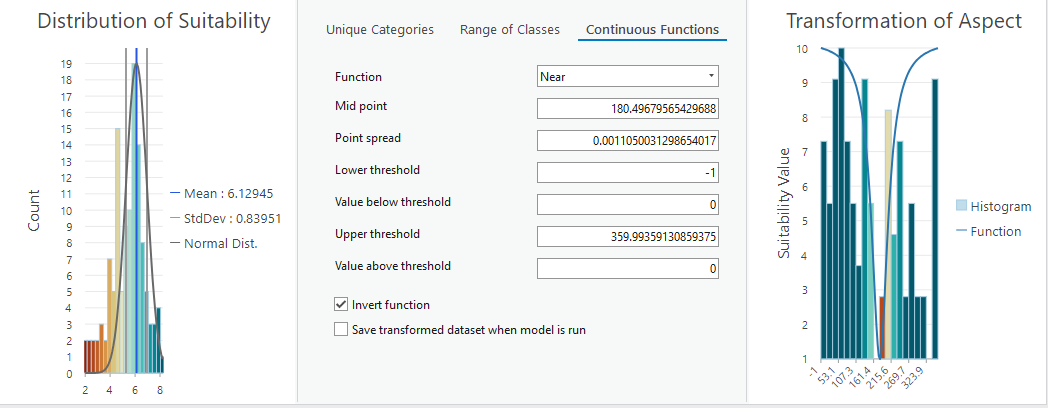
\includegraphics{images/Aspect_suitability.PNG}

}

\caption{Screenshot of Transfer function for Aspect Suitability}

\end{figure}%

\begin{center}\rule{0.5\linewidth}{0.5pt}\end{center}

\subparagraph{Slope}\label{slope}

Higher slopes are less suitable because thinning is both more expensive,
and more precipitation will end up as runoff.

\begin{quote}
Lower slopes have higher suitability scores
\end{quote}

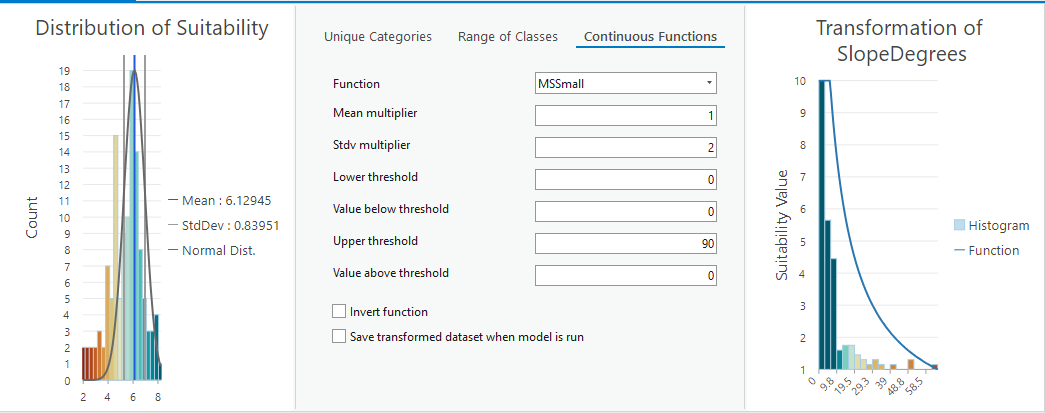
\includegraphics{images/Slope_suitability.PNG}

\begin{center}\rule{0.5\linewidth}{0.5pt}\end{center}

\subparagraph{Elevation}\label{elevation}

Water yield in lower elevation watersheds will be less responsive to
changes in forest structure due to asynchrony between snowmelt and
transpiration \citep{biederman2022}

Winter precipitation mainly falls as snow at elevations above 1800m in
Arizona \citep{friederici2013}

\begin{center}\rule{0.5\linewidth}{0.5pt}\end{center}

\subparagraph{Precipitation}\label{precipitation}

\begin{quote}
\textbf{Ideal:} Mean annual precipitation must be higher than 500mm 1990
- 2020

\textbf{Marginal:} (benefits only expected in wet years or during some
events) Max precipitation higher than 500mm but Mean annual
precipitation \textless{} 500mm

\textbf{Unsuitable:} Max annual precipitation \textless{} 500mm
\end{quote}

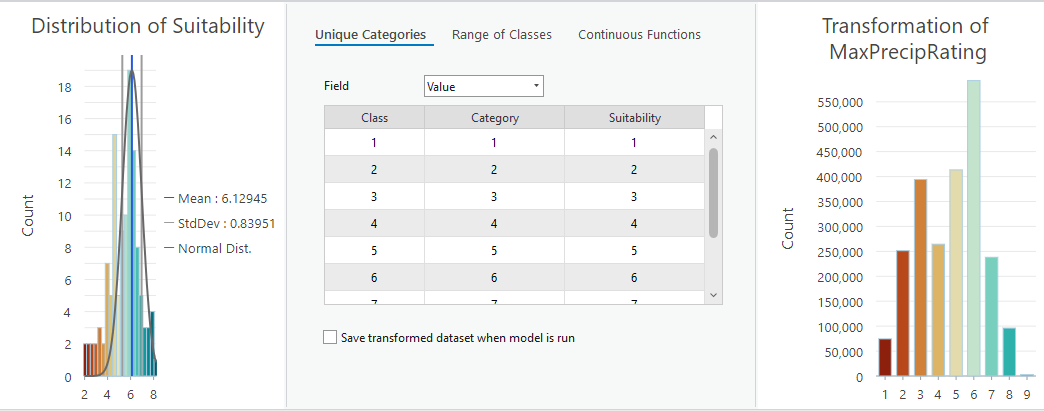
\includegraphics{images/Precipitation_suitability.PNG}

\begin{center}\rule{0.5\linewidth}{0.5pt}\end{center}

\subparagraph{Vegetation
Characteristics}\label{vegetation-characteristics}

Higher vegetation density, when thinned, will yield more water, so focus
on areas of high vegetation density and high departure from historic
conditions.

\begin{quote}
\textbf{NLCD 2021 Total Canopy Cover (\% Cover)}
\end{quote}

\begin{quote}
Canopy cover \% below 30 were considered low suitability (1) while
increases in canopy cover about 30\% increase in suitability.
\end{quote}

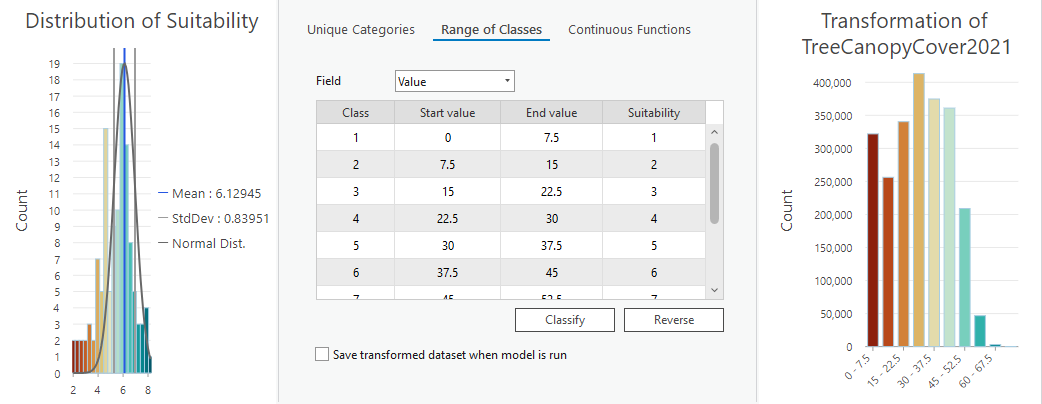
\includegraphics{images/CanopyCover_suitability.PNG}

\begin{quote}
\textbf{Landfire 2022 Vegetation Condition Class} 3rd update to the 2016
remap.
\end{quote}

Variation from modeled historic conditions. Forests that have deviated
significantly from their modeled historic conditions are more suitable
for thinning than forests that have not deviated from their historic
condition.

\begin{quote}
Vegetation Condition Class (VCC) represents a simple categorization of
the associated Vegetation Departure (VDep) and is a derivative of the
VDep layer. It indicates the general level to which current vegetation
differs from the estimated modeled vegetation based on past reference
conditions. VDep and VCC are based upon methods originally described in
the Inter-agency Fire Regime Condition Class Guidebook but are not
identical to those methods. They should not be considered as a
replacement data set. Full descriptions of the techniques used can be
found in the VDep product description. Note that the LANDFIRE (LF) team
feels it is very important for users to review the VDep methods before
comparing VDep or VCC values across LF versions.
\href{https://www.landfire.gov/vegetation/vcc}{info}
\href{https://www.landfire.gov/sites/default/files/DataDictionary/LF2022/LF22_VCCADD_230.pdf}{PDF}
\end{quote}

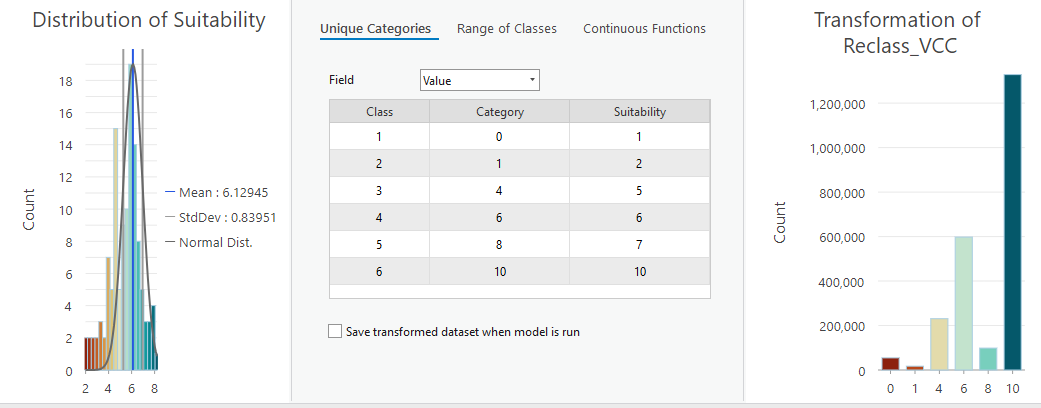
\includegraphics{images/VCC_suitability.PNG}

\begin{center}\rule{0.5\linewidth}{0.5pt}\end{center}

\subparagraph{Soil Hydrologic
Conditions}\label{soil-hydrologic-conditions}

Soil types A,B,C,D are mapped for the USA, There are no A soil types in
the study area, so they were given the following suitability values

B = 10 out of 10 C = 8 out of 10 D = 3 out of 10

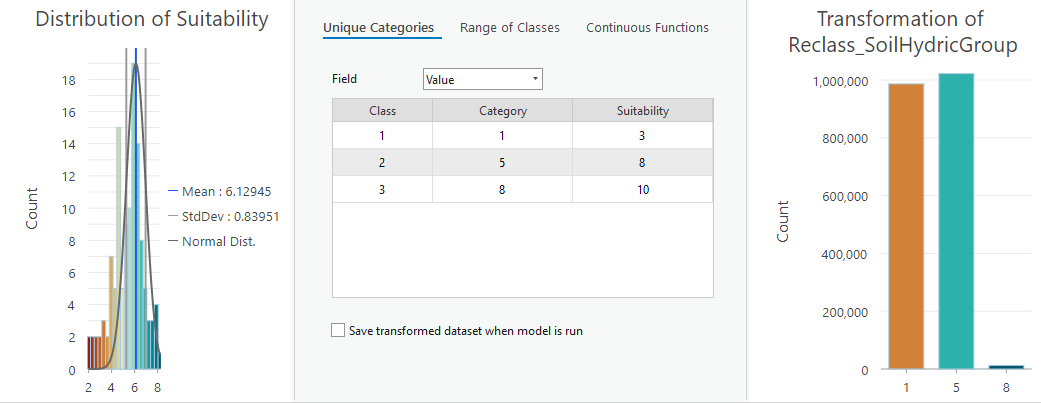
\includegraphics{images/SoilHydrologicGroup_suitability.PNG}

\subsection{Preliminary Results}\label{preliminary-results}

\subsubsection{Weighting}\label{weighting}

Tree Canopy Cover = 20\% Vegetation Condition Class = 20\% Slope = 20\%
Aspect = 20\% Max Precipitation = 15\% Soil Hydrologic Group = 5\%

\subsubsection{Overall Suitability}\label{overall-suitability}

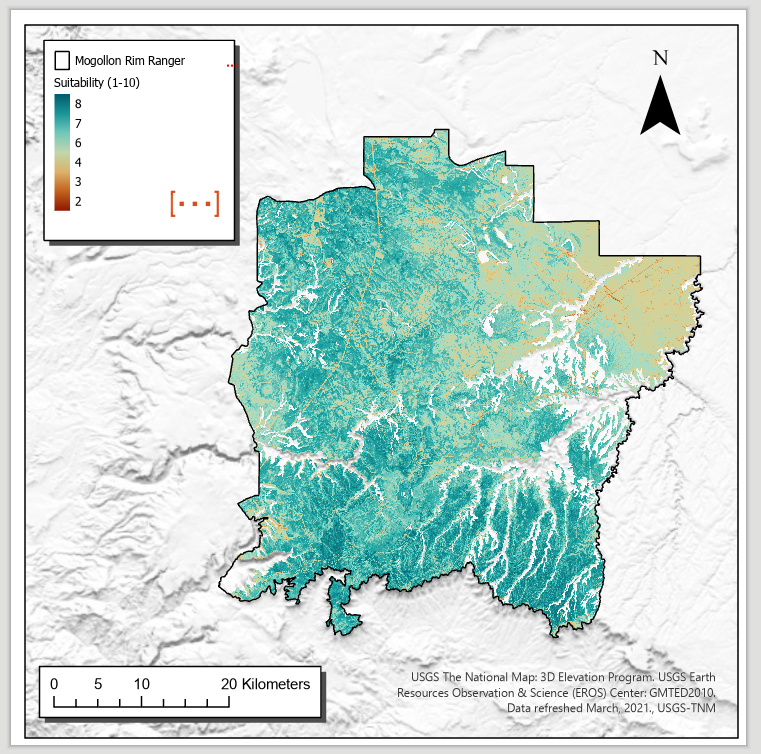
\includegraphics{images/PreliminarySuitabilityMap.PNG}

\subsection{Acknowledgments}\label{acknowledgments}

Phasellus interdum tincidunt ex, a euismod massa pulvinar at. Ut
fringilla ut nisi nec volutpat. Morbi imperdiet congue tincidunt.
Vivamus eget rutrum purus. Etiam et pretium justo. Donec et egestas sem.
Donec molestie ex sit amet viverra egestas. Nullam justo nulla,
fringilla at iaculis in, posuere non mauris. Ut eget imperdiet elit.

\subsection{Open research}\label{open-research}

Phasellus interdum tincidunt ex, a euismod massa pulvinar at. Ut
fringilla ut nisi nec volutpat. Morbi imperdiet congue tincidunt.
Vivamus eget rutrum purus. Etiam et pretium justo. Donec et egestas sem.
Donec molestie ex sit amet viverra egestas. Nullam justo nulla,
fringilla at iaculis in, posuere non mauris. Ut eget imperdiet elit.

\subsection*{References}\label{references}
\addcontentsline{toc}{subsection}{References}

\renewcommand{\bibsection}{}
\bibliography{bibliography.bib}




\end{document}
